%https://pt.quora.com/Como-encontrar-todos-os-n%C3%BAmeros-inteiros-positivos-a-e-b-de-modo-que-ab-seja-divis%C3%ADvel-por-a-b

%https://math.stackexchange.com/questions/2775233/does-dn-always-depend-on-gcdn-sigman-when-sigman-anb-n-xn

%https://math.stackexchange.com/questions/3073053/if-sigman-2n-d-and-d-mid-n-is-it-true-that-d-gcdn-sigman?rq=1



%http://math.mit.edu/~drew/
%https://math.stackexchange.com/questions/93689/software-for-galois-theory
%SetClassGroupBounds("GRH"); 
%K := QuadraticField(9);
%ClassNumber(K);

%https://en.wikipedia.org/wiki/List_of_triangle_inequalities

\documentclass[12pt, a4paper]{article}
\usepackage[bottom=2cm,top=3cm,left=3cm,right=2cm]{geometry}
\usepackage[utf8]{inputenc}
\usepackage{CJKutf8}
\usepackage{mathtext}
\usepackage{graphicx}
\usepackage{wrapfig}
\usepackage[T1]{fontenc}
\usepackage{blindtext}
\usepackage{tasks}
\usepackage{setspace}
\usepackage{amsmath}
\usepackage{amsfonts}
\usepackage{amssymb}
\usepackage{ wasysym }
\usepackage[portuguese]{babel}
\usepackage[utf8]{inputenc}
\usepackage{mathtext}
\usepackage{graphicx}
\usepackage{wrapfig}
\usepackage[T1]{fontenc}
\usepackage{blindtext}
\usepackage{setspace}
\usepackage{amsmath}
%\usepackage{geometry}
\usepackage{amsthm}
\usepackage{graphics}
%\usepackage{amsfonts}
%\usepackage{lipsum}
\usepackage{amssymb}
\usepackage{CJKutf8} %Pacote para escrever em japonês \begin{CJK}{UTF8}{min} \end{CJK}
\usepackage[portuguese]{babel}
\usepackage{multicol}
% \usepackage{colorspace}
\usepackage{graphicx, color}
\newcommand{\mdc}{{\rm mdc}}
\newcommand{\sen}{{\rm sen}}
\newcommand{\tg}{{\rm tg}}
\newcommand{\cotg}{{\rm cotg}}
\newcommand{\cossec}{{\rm cossec}}
\newcommand{\arctg}{{\rm arctg}}
\newcommand{\arcsen}{{\rm arcsen}}
\newcommand{\pulaquestao}{\newline\newline}
\newcommand{\negrito}[1]{\mbox{\boldmath{$#1$}}} 
\usepackage{pifont}
\newcommand{\heart}{\ensuremath\heartsuit}
\newcommand{\diamonde}{\ensuremath\diamondsuit}
\newtheorem{defi}{Definição}
\newtheorem{propo}{Proposição}
\newtheorem{dem}{Demonstração}
\newtheorem{coro}{Corolário}
\DeclareSymbolFont{extraup}{U}{zavm}{m}{n}
\DeclareMathSymbol{\varheart}{\mathalpha}{extraup}{86}
\DeclareMathSymbol{\vardiamond}{\mathalpha}{extraup}{87}
\setlength{\parindent}{0pt}
\usepackage[framemethod=TikZ]{mdframed}
%\usepackage{lipsum}
\mdfdefinestyle{MyFrame}{%
    linecolor=blue,
    outerlinewidth=2pt,
    roundcorner=20pt,
    innertopmargin=\baselineskip,
    innerbottommargin=\baselineskip,
    innerrightmargin=20pt,
    innerleftmargin=20pt,
    backgroundcolor=white!50!white}
    
%\mdfdefinestyle{Solução}{%
%    linecolor=blue,
%    outerlinewidth=1pt,
%    roundcorner=8pt,
%    innertopmargin=4pt%\baselineskip,
%    innerbottommargin=0pt%\baselineskip,
%    innerrightmargin=20pt,
%    innerleftmargin=20pt,
%    backgroundcolor=white!50!white}
    
    
    \mdfdefinestyle{DAS}{%
    linecolor=blue,
    outerlinewidth=2pt,
    roundcorner=20pt,
    innertopmargin=\baselineskip,
    innerbottommargin=\baselineskip,
    innerrightmargin=20pt,
    innerleftmargin=20pt,
    backgroundcolor=white!50!green}
% \definespotcolor{mygreen}{PANTONE 7716 C}{.83, 0, .00, .51}
% \definespotcolor{tuti}{}{0.6, 0, 1, .508}
\title{PIC - Programa de Iniciação Científica}
\author{Douglas de Araujo Smigly}
\date{29 de agosto de 2020}
\begin{document}
\definecolor{Floresta}{rgb}{0.13,0.54,0.13}
\maketitle
\begin{center}
\large\textbf{\textcolor{Floresta}{Ciclo 4 - Encontro 1 - Aritmética}}\\
\end{center}
%\begin{multicols*}{2}
%\setlength{\columnseprule}{0.78pt}
%\raggedcolumns
%\columnbreak
\textcolor{blue}{\bf(1)} (OBMEP 2006) O número $abcde$ tem cinco algarismos distintos e diferentes de zero, cada um deles
representado por uma das letras $a, b, c, d, e.$ Multiplicando-se este número por $4,$
obtém-se número de cinco algarismos $edcba.$ Qual é o valor de $a + b + c + d + e?$
\newline\newline
\textcolor{blue}{\bf(2)} (OBMEP 2007) O \textit{contrário }de um número de dois algarismos, ambos diferentes de zero, é o número
obtido trocando-se a ordem de seus algarismos. Por exemplo, o contrário de $25$ é $52$ e o contrário de $79$ é $97.$ Qual dos números abaixo não é soma de um número de dois algarismos com seu contrário?
\begin{tasks}[counter-format={(tsk[a])},label-width=3.6ex, label-format = {\bfseries}, column-sep = {0pt}](5)
\task[\textcolor{Floresta}{$\negrito{(a)} $}] $44$
\task[\textcolor{Floresta}{$\negrito{(b)} $}] $99$
\task[\textcolor{Floresta}{$\negrito{(c)} $}] $121$
\task[\textcolor{Floresta}{$\negrito{(d)} $}] $165$
\task[\textcolor{Floresta}{$\negrito{(e)} $}] $181$
\end{tasks} 
\textcolor{blue}{\bf(3)} (OBMEP 2012) Um quadrado de lado $1$ cm roda em torno de um quadrado de lado $2$ cm, como na
figura abaixo, partindo da posição inicial e completando um giro cada vez que um de seus lados fica apoiado em um lado do quadrado maior. Como ficaria a figura que representa a posição dos dois quadrados após o $2012^\circ$ giro?
\begin{figure}[!h]
    \centering
    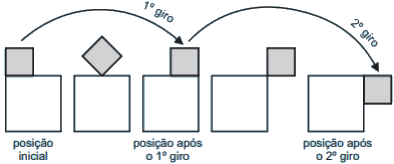
\includegraphics{Figuras/q3c4e1.png}
\end{figure}


\textcolor{blue}{\bf(4)} (OBMEP 2013) Marcos fez cinco provas de Matemática. Suas notas, em ordem crescente, foram $75,80, 84, 86$ e $95.$ Ao digitar as notas de Marcos na ordem em que as provas foram realizadas, o professor notou que as médias das duas primeiras provas, das três primeiras, das quatro primeiras e das cinco provas eram números inteiros. Qual foi a nota que Marcos tirou na última prova?
\newline\newline
\textcolor{blue}{\bf(5)} (OBMEP 2015) Uma sequência de números é definida por $a_1 = 3$ e $a_{n+1} = a_n + a_n^2, \forall n \ge 1.$ Por exemplo, $a_2 = a_1 + a_1^2 = 3 + 3^2 = 12.$ Qual é o algarismo das unidades de $a_{2015}?$
\newline\newline
\textcolor{blue}{\bf(6)} (OBMEP 2017) Somando $1$ a um certo número natural, obtemos um múltiplo de $11.$ Subtraindo 1 desse mesmo número, obtemos um múltiplo de $8.$ Qual é o resto da divisão do quadrado desse número por $88?$
\newline\newline
\textcolor{blue}{\bf(7)} (Banco de Questões - OBMEP 2010) Escreve-se em ordem crescente os múltiplos de $3$ que, somados com $1,$ sejam quadrados perfeitos, ou seja, $3, 15, 24, 48, \ldots$ Qual é o múltiplo de $3$ na 2006ª posição?
\newline\newline
\textcolor{blue}{\bf(8)} (Banco de Questões - OBMEP 2015) O mágico Magimático diz para uma pessoa da plateia escolher uma peça qualquer de um dominó comum. Tal peça é formada por um par de números de $0$ a $6.$ Em seguida, ele diz para a pessoa escolher um dos números da peça e realizar a seguinte sequência
de operações:
\begin{enumerate}
    \item multiplicá-lo por $5;$
\item somar o resultado anterior com $15;$
\item multiplicar o último resultado por $2$ e, finalmente,
\item somar o último resultado com o outro número da peça.
\end{enumerate}
Realizadas tais operações, o resultado é divulgado e Magimático impressiona a plateia dizendo exatamente os números escritos no dominó escolhido.
\begin{tasks}[counter-format={(tsk[a])},label-width=3.6ex, label-format = {\bfseries}, column-sep = {0pt}](1)
\task[\textcolor{Floresta}{$\negrito{(a)} $}] Sabendo que o resultado foi $62,$ como o mágico descobriu o número escolhido pelo membro da plateia?
\task[\textcolor{Floresta}{$\negrito{(b)} $}] Se o resultado tivesse sido $n,$ como descobrir os números da peça escolhida?
\end{tasks}
\textcolor{blue}{\bf(9)} São colocados nove números em um círculo: quatro iguais a $1$ e cinco iguais a zero. Efetua-se a seguinte operação nos números: entre cada par de números adjacentes coloca-se um zero se os números forem diferentes e um $1$ se forem iguais. Depois, apaga-se os números ``velhos''. Depois desta operação ser efetuada diversas vezes, é possível que todos os números sejam iguais?
\newline
\newline
\textcolor{blue}{\bf(10)} Um número foi obtido permutando-se os algarismos de outro número.
\begin{tasks}[counter-format={(tsk[a])},label-width=3.6ex, label-format = {\bfseries}, column-sep = {0pt}](1)
\task[\textcolor{Floresta}{$\negrito{(a)} $}] A soma desses dois números pode ser igual a $9999?$
\task[\textcolor{Floresta}{$\negrito{(b)} $}] A soma desses dois números pode ser igual a $99999?$
\end{tasks}

\textcolor{blue}{\bf(11)} A soma dos algarismos de $100! = 1 \times 2 \times 3 \ldots \times 100$  foi escrita na representação decimal. A soma dos algarismos do número resultante foi escrita na representação decimal, e assim por diante. Finalmente, o resultado é um número de um único algarismo. Encontre esse número.
\newline\newline
\textcolor{blue}{\bf(12)} Suponhamos que temos sete números naturais tais que a soma de seis quaisquer deles é divisível por $5.$ Cada um dos sete números tem que ser, necessariamente, divisível por $5?$\newline \newline
\textcolor{blue}{\bf(13) $\varheart$} Prove que é impossível encontrar $9$ números que somem $2020$ e cujo antecessor é múltiplo de $3.$ 
\newline\newline
\textcolor{blue}{\bf(14) $\varheart$} Em um tabuleiro de xadrez, um cavalo sai da posição $a1$ e retorna para a mesma posição depois de vários movimentos. Mostre que o cavalo fez um número par de movimentos.
 
\begin{center}
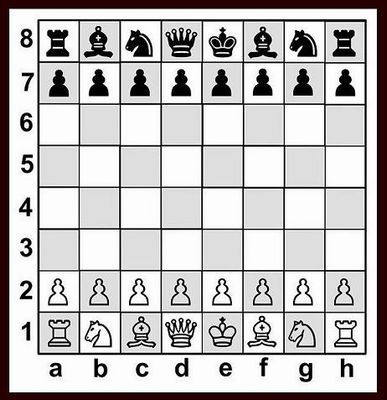
\includegraphics[scale=0.5]{Listas do PIC/xadrez.jpg}
\end{center}

%https://artofproblemsolving.com/community/c6h473647p2651848
\textcolor{blue}{\bf(15) $\varheart$} Cinco amigos compraram uma pizza grande e a dividiram em $14$ pedaços. Prove que um número ímpar de amigos comeu um número par de pedaços.
\newline\newline
\textcolor{blue}{\bf(16) $\varheart$} No reino da Frutilândia existe uma árvore mágica que possui $2019$ maçãs e $2020$ tomates. Todo dia um garoto sobe na árvore e come duas frutas. Quando ele come duas frutas iguais, nasce um tomate na árvore; quando ele come duas frutas diferentes, nasce uma maçã. Após alguns dias restará apenas uma fruta na árvore. Que fruta será?
\begin{center}
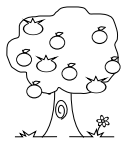
\includegraphics[scale=1]{Listas do PIC/frutilandia.png}
\end{center}
\textcolor{blue}{\bf(17) $\varheart$} (Ucrânia 1997) Considere um tabuleiro pintado de preto e branco da maneira usual e, em cada casa do tabuleiro, escreva um número inteiro, de modo que a soma
dos números em cada coluna e em cada linha é par. Mostre que a soma dos números nas casas pretas é par.
\newline\newline
\textcolor{blue}{\bf(18) $\varheart$} (Critério de divisibilidade por $7$) Para verificar se um número é divisível por $7$, devemos duplicar o algarismo das unidades e subtrair o resto do número. Se o resultado dessa operação for divisível por $7,$ então o número é divisível por $7.$
\begin{tasks}[counter-format={(tsk[a])},label-width=3.6ex, label-format = {\bfseries}, column-sep = {0pt}](1)
\task[\textcolor{Floresta}{$\negrito{(a)} $}] Verifique se os números $56735,$ $1563$ e $1057$ são divisíveis por $7$.
\task[\textcolor{Floresta}{$\negrito{(b)} $}] Prove a validade desse critério de divisibilidade para números de $4$ algarismos.
\end{tasks}
\textcolor{blue}{\bf(19) $\varheart$} (Critério de divisibilidade por $13$) Para verificar se um número é divisível por $13$, devemos quadruplicar o algarismo das unidades e subtrair o resto do número. Se o resultado dessa operação for divisível por $13,$ então o número é divisível por $13.$
\begin{tasks}[counter-format={(tsk[a])},label-width=3.6ex, label-format = {\bfseries}, column-sep = {0pt}](1)
\task[\textcolor{Floresta}{$\negrito{(a)} $}] Verifique se os números $15632,$ $125465645$ e $49049$ são divisíveis por $13$.
\task[\textcolor{Floresta}{$\negrito{(b)} $}] Prove a validade desse critério de divisibilidade para números de $4$ algarismos.
\end{tasks}
\textcolor{blue}{\bf(20) $\varheart$} Encontre um número $d$ que satisfaça o seguinte critério de divisibilidade:
\textit{Para verificar se um número é divisível por $d$, devemos octuplicar (multiplicar por $8$) o algarismo das unidades e subtrair o resto do número. Se o resultado dessa operação for divisível por $d,$ então o número é divisível por $d.$}%81,pois 10*8=-1mod81
\newline\newline
\textcolor{blue}{\bf(21) $\varheart$} Dado um número natural positivo $n,$ dizemos que um número $m$ é \textbf{resíduo quadrático módulo} $n$ se existe um número $x$ tal que o resto da divisão de $x^2$ por $n$ é $m.$ Por exemplo, $4$ é um resíduo quadrático módulo $7,$ pois $5^2 = 25$ deixa resto $4$ na divisão por $7.$
\begin{tasks}[counter-format={(tsk[a])},label-width=3.6ex, label-format = {\bfseries}, column-sep = {0pt}](1)
\task[\textcolor{Floresta}{$\negrito{(a)} $}] Encontre todos os resíduos quadráticos módulo $6.$
\task[\textcolor{Floresta}{$\negrito{(b)} $}] Um número quadrado perfeito pode terminar em $7$? Justifique sua resposta.
\end{tasks}
\textcolor{blue}{\bf(22) $\varheart$} A soma de $3$ números é $100,$ dois são primos e um é a soma dos outros dois.
\begin{tasks}[counter-format={(tsk[a])},label-width=3.6ex, label-format = {\bfseries}, column-sep = {0pt}](1)
\task[\textcolor{Floresta}{$\negrito{(a)} $}] Qual é o maior dos 3 números?
\task[\textcolor{Floresta}{$\negrito{(b)} $}] Dê um exemplo desses 3 números.
\task[\textcolor{Floresta}{$\negrito{(c)} $}] Quantas soluções existem para esse problema?
\end{tasks}
\textcolor{blue}{\bf(23) $\varheart$} Um gafanhoto vive na reta coordenada. Inicialmente, ele se encontra no ponto $1.$ Ele pode pular $1$ ou $5$ unidades, tanto para direita quanto para esquerda. Porém, a reta coordenada possui buracos em todos os pontos que são múltiplos de $4$ (i.e. existem buracos nos pontos $-4, 0, 4, 8$ etc), então ele não pode pular para estes pontos. Pode o gafanhoto chegar ao ponto $3$ após $2003$ saltos?
\begin{center}

\includegraphics[scale=1.5]{Listas do PIC/gafanhoto.png}
\end{center}

Exercícios marcados com $\varheart$ são extras.
\end{document}
SetClassGroupBounds("GRH"); 
K := QuadraticField(9);
ClassNumber(K);
Q := PolynomialRing(GF(2), 2);
Q;
K := QuadraticField();
G := GaloisGroup(K);
G;
\begin{CJK}{UTF8}{min}
露の世は 露の世ながら さりながら当時では老人と呼べる50歳代半ばでようやく授かったわが子への愛とその突然死を伝えた「露の世」のくだりは、その日記体句文集「おらが春」のクライマックスとなっています。

5月には数え二歳の誕生を迎えて詠んだ句に、
「這へ笑へ二つになるぞけさからは」と喜びを謳歌したばかり。

それが、翌6月にはもはや草葉の陰へと、その露の朝日に立ちどころに消えるごとく、儚くも身罷ってしまったとは。

人の世は朝露の如く無常なのだと、悔みを述べ慰問するあの人、この人。さは「さりながら」…それは確かにそうなのだけれども。
いかに「あきらめ顔しても、思い切りがたきは、恩愛のきづな也けり。」と、わが心中は耐えきれず切々と泣き崩れるばかり。わが子「さと」女を思う「大切」はやがて「あなた任せ」の境地へと通じていくものでしょう。
\end{CJK}